\chapter{Tool usage and extension guides}

Consult this chapter to learn how to use and extend of ModularDoc.

In the context of this thesis ModularDoc was developed with only one plugin - \ref{gloss:markdown} for \ref{gloss:git}.
Thus, the user guide covers the tool with this plugin in mind.

The extension guide is designated for those, who wish to extend ModularDoc with new components, or plugin. ModularDoc also allows other areas of the application to be modified; however, due to the complexity and low necessity of these modifications, their description will be omitted from this guide.

\begin{figure}[H]
    \dirtree{%
    .1 ~ModularDocInstallationRoot/.
    .2 ModularDoc.App.exe.
    .2 Components/.
    .2 Libraries/.
    .2 Plugins/.
    .3 GitMarkdown/.
    .4 ModularDoc.Plugins.GitMarkdown.dll.
    .4 ....
    .2 ....
    }
    \caption{ModularDoc simplified file and folder structure}
    \label{fig:applicationFileStructure}
\end{figure}

\section{User guide}

ModularDoc is delivered as a portable application without an installer. Thus, mentioned files and folders are in the context of the ones either provided with this thesis, or compiled from the source code (see figure \ref{fig:applicationFileStructure}). The source code is also provided with this thesis; however, the most up-to-date version can be found on GitHub (see \Nameref{sec:openSource}).

\subsection{Prerequisites}

\begin{itemize}
    \item A desktop device running either of the following \ref{itm:os}'s:
    \begin{itemize}
        \item Windows 7+
        \item macOS High Sierra 10.13+\footnote{ModularDoc was not tested on a macOS device, due to lack of Apple hardware}
        \item  Debian 9 (Stretch)+, Fedora 30+, or Ubuntu 16.04+ (Linux distribution with \textit{glibc} 2.17 installed, or a newer version)\footnote{ModularDoc was tested on PopOS 22.04 LTS, a Linux distribution from system76}
    \end{itemize}
    \item The \ref{itm:os} must be 64bit
    \item \ref{gloss:dotnetlabel} Runtime 6.0.11+ is installed
    \item Free 270 MB of disk space
\end{itemize}

\subsection{ModularDoc application}

The ModularDoc application can be started by running the \textit{ModularDoc.App.exe} file (see figure \ref{fig:applicationFileStructure}).

\subsubsection{Home page}

Within the application, the user can selected one of the available plugins and start configuring it via the configuration stepper, then running and saving the configuration in the summary.
Additionally, the user can load the created configuration, edit it or just run it.

\begin{figure}[H]
    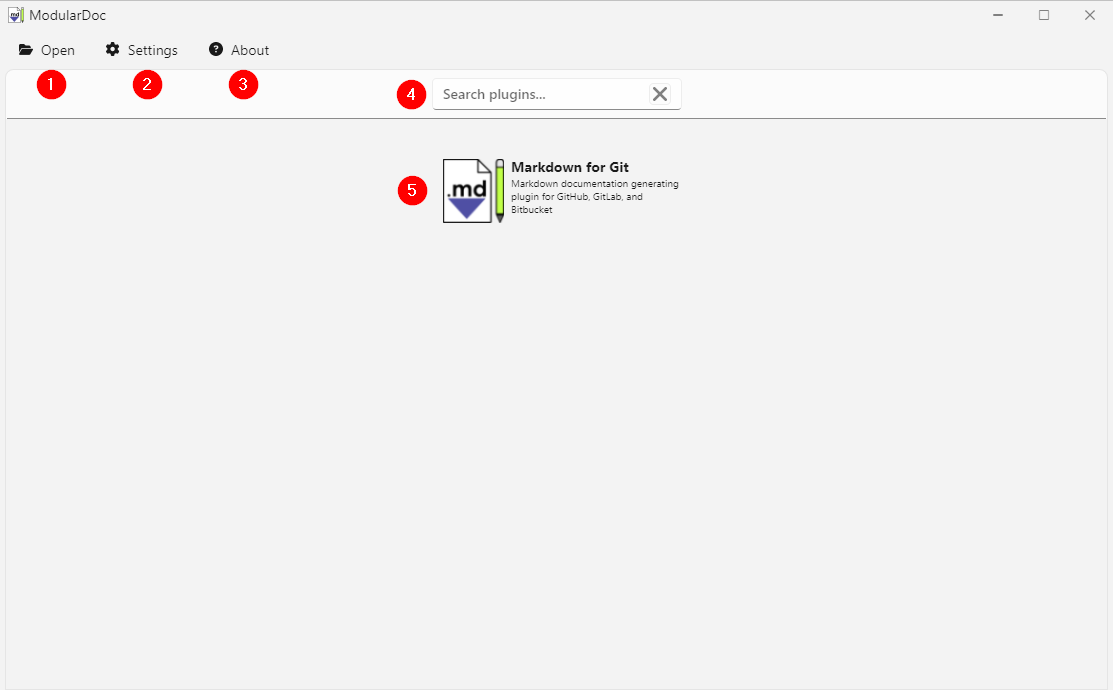
\includegraphics[width=\linewidth]{img/modularDocHomePage.png}
    \label{fig:modularDocHome}
    \caption{ModularDoc home page}
\end{figure}

\begin{enumerate}
    \item Open button for loading previously defined configurations
    \item Settings button for navigating to the settings page
    \item About button for displaying information about the application
    \item Search entry for filtering the available plugins
    \item One of the available plugins with its icon, title, and short description
\end{enumerate}

\begin{figure}[H]
    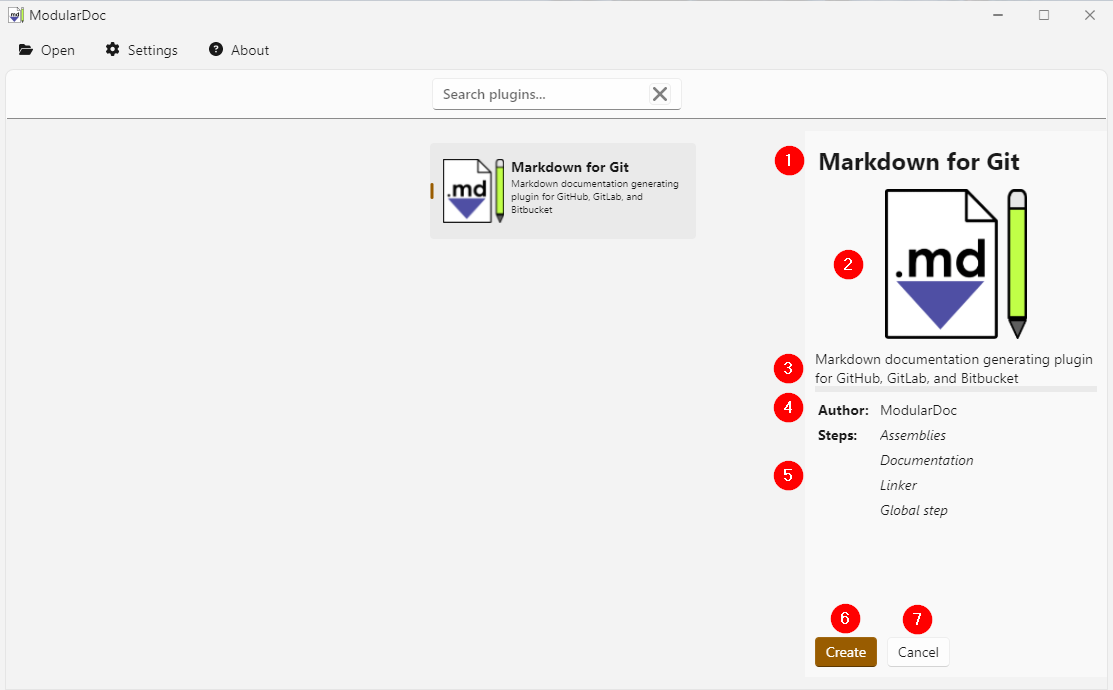
\includegraphics[width=\linewidth]{img/modularDocPluginSelected.png}
    \label{fig:modularDocPluginSelected}
    \caption{ModularDoc home page with a plugin selected}
\end{figure}

\begin{enumerate}
    \item Plugin title
    \item Plugin icon
    \item Plugin description
    \item Author information
    \item Steps within said plugin
    \item Button for creating a configuration using the selected plugin
    \item Button for closing the selected plugin panel
\end{enumerate}

\pagebreak
\subsubsection{Configuration wizard}

The configuration wizard presents the selected plugin's steps. Each step's settings are displayed for configuration. The user can view additional help for each active step. Navigating to the next step is possible only is the active one is configured correctly.

\begin{figure}[H]
    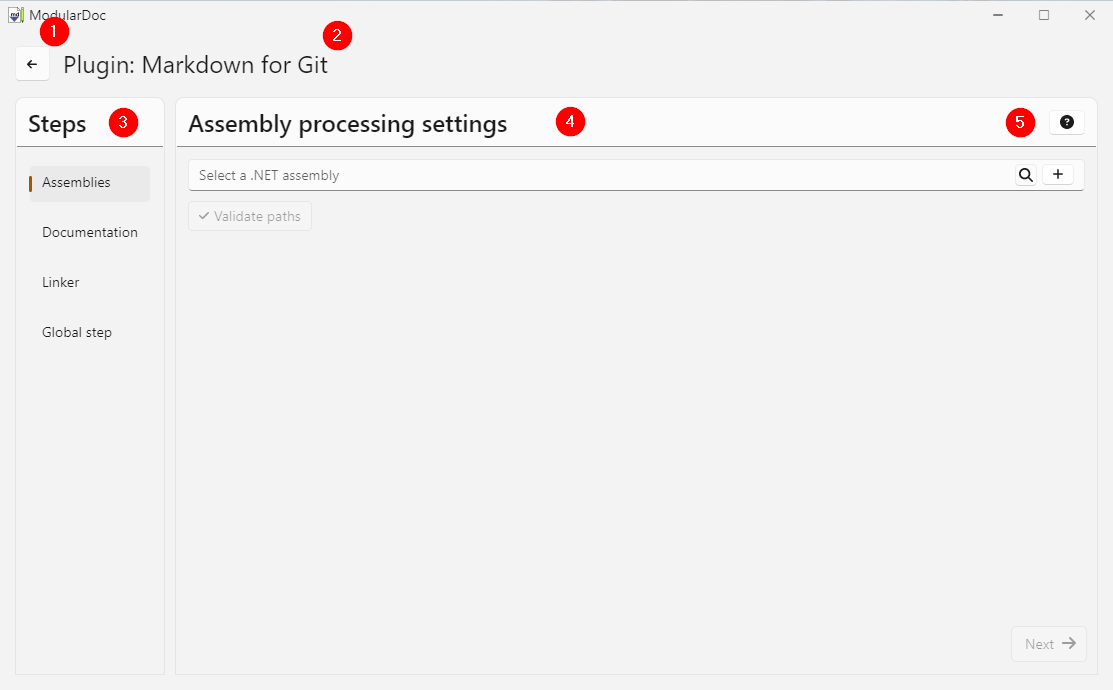
\includegraphics[width=\linewidth]{img/modularDocConfigurator.png}
    \label{fig:modularDocconfiguratorPage}
    \caption{ModularDoc configuration wizard}
\end{figure}

\begin{enumerate}
    \item Back button for navigating back to the home page
    \item Title of the plugin
    \item List of steps provided by the plugin, with the current step highlighted
    \item The current step configuration title and view
    \item Information for the user to help them configure the step correctly
\end{enumerate}

\pagebreak
\subsubsection{Summary page}

Completing the last plugin step navigates to the summary page, which executes the plugin using the created configuration. The execution processes are displayed, alongside their progress. Each process logs messages, that can be grouped by the process source and log type. At this stage, it is possible to save the configuration, go back to the configuration wizard, or return to the home page.

\begin{figure}[H]
    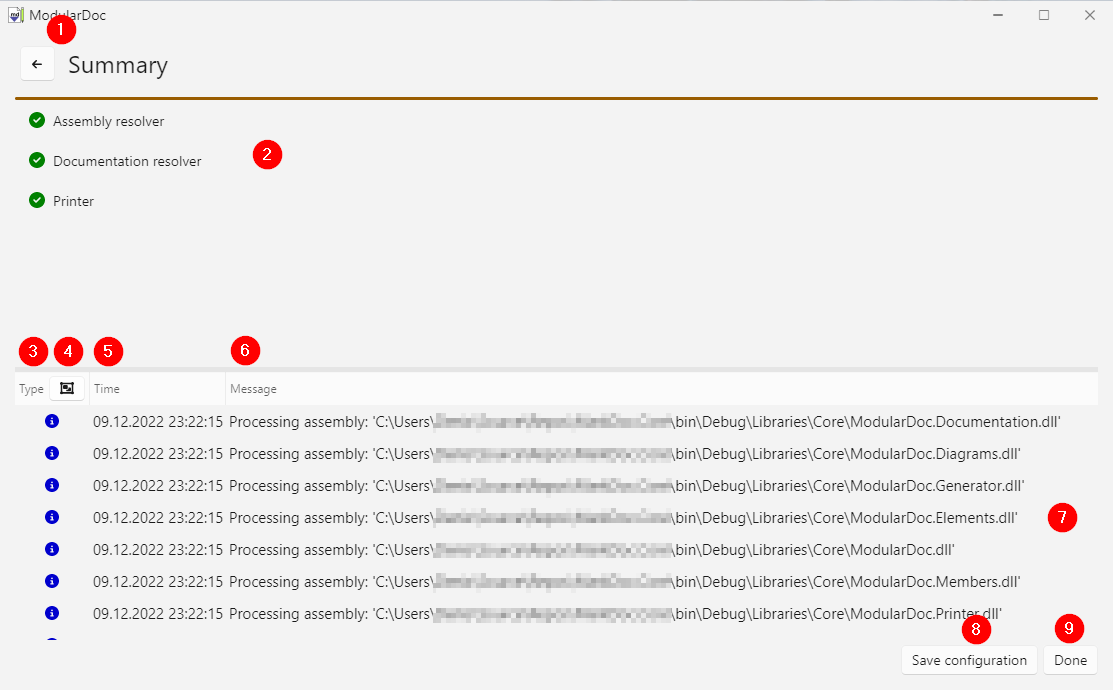
\includegraphics[width=\linewidth]{img/modularDocSummary.png}
    \label{fig:modularDocSummaryPage}
    \caption{ModularDoc summary}
\end{figure}

\begin{enumerate}
    \item Back button for navigating back to the configurator
    \item List of executed processes, their states
    \item Type of logged message
    \item Log message grouping options
    \item Time of logged message
    \item Log message text
    \item Log messages
    \item Button for saving the created configuration
    \item Button for returning back to the home page
\end{enumerate}

\begin{figure}[H]
    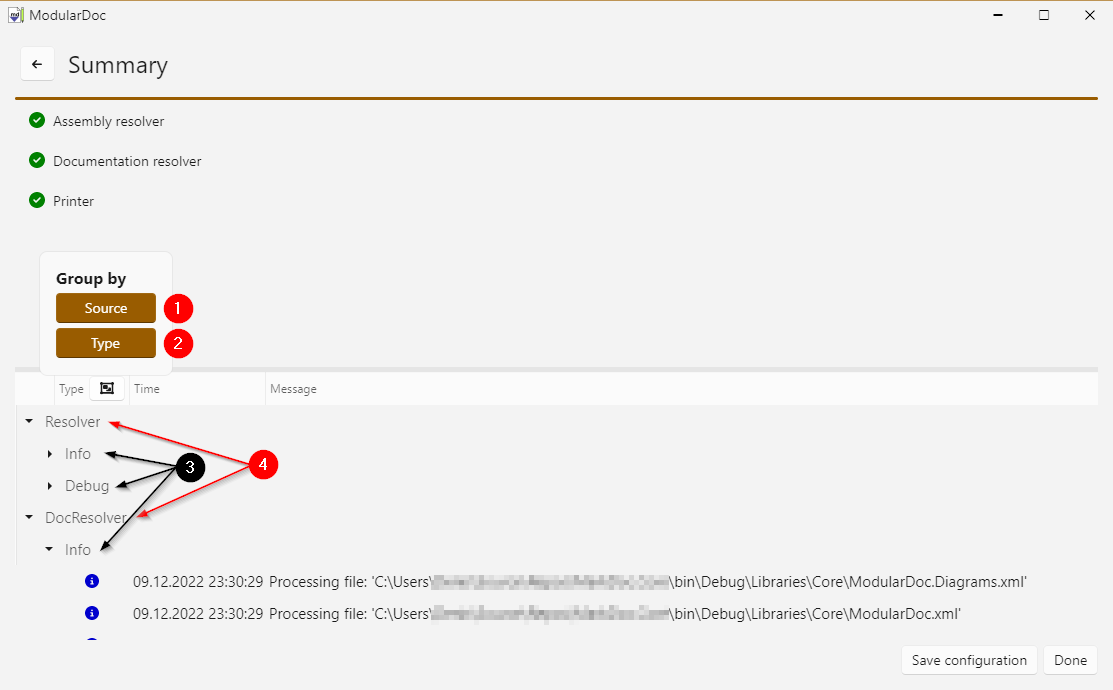
\includegraphics[width=\linewidth]{img/modularDocSummaryLogGroupping.png}
    \label{fig:modularDocSummaryGroupingPage}
    \caption{ModularDoc summary log grouping}
\end{figure}

\begin{enumerate}
    \item Toggle for grouping by message source
    \item Toggle for grouping by message type
    \item Groups by message type
    \item Groups by message source
\end{enumerate}

\pagebreak
\subsubsection{Settings page}

The applications settings allow the user to toggle its theme between dark mode and light mode.

\begin{figure}[H]
    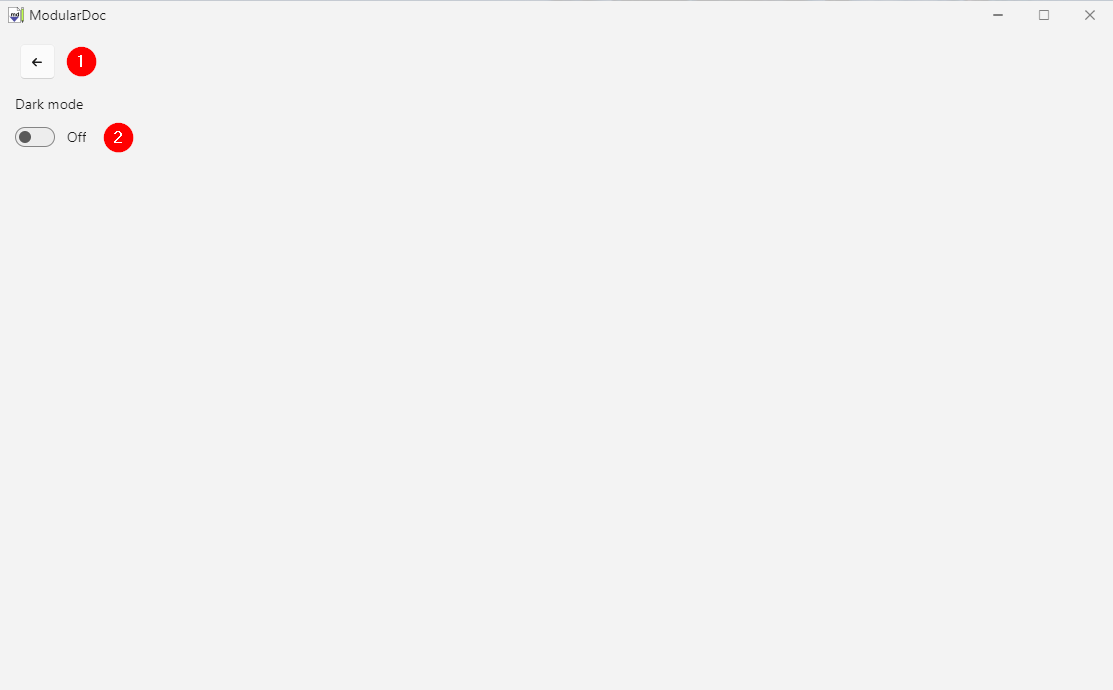
\includegraphics[width=\linewidth]{img/modularDocSettings.png}
    \label{fig:modularDocSettingsPage}
    \caption{ModularDoc settings page}
\end{figure}

\begin{enumerate}
    \item Back button for navigating back to the home page
    \item Toggle switch for changing the theme from light mode to dark mode
\end{enumerate}

\pagebreak
\subsection{Markdown for Git plugin}

The \ref{gloss:markdown} for \ref{gloss:git} plugin is designed specifically for processing \ref{gloss:dotnetlabel} libraries written in C\# and outputting developer documentation in \ref{gloss:markdown} form suitable for \ref{gloss:git} platforms such as GitHub or GitLab.

\subsubsection{Assemblies step}

The assemblies step is designated for selecting file paths to \ref{gloss:dotnetlabel} assemblies or executables for processing. It is possible to proceed to the next step only after providing at least one file path.

\begin{figure}[H]
    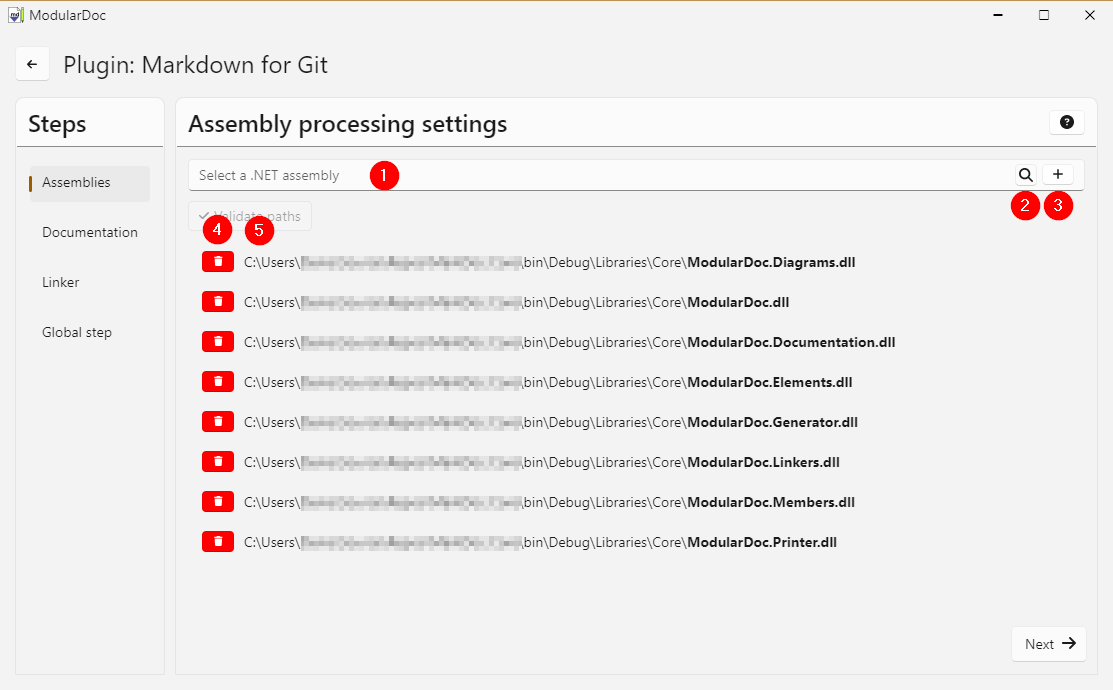
\includegraphics[width=\linewidth]{img/modularDocAssemblies.png}
    \label{fig:modularAssemblies}
    \caption{Plugin assembly configuration step}
\end{figure}

\begin{enumerate}
    \item Input field for supplying a file path
    \item Button for opening the file browser and selecting file paths
    \item Button for adding the supplied path via the input field, or opening the file browser (see 2) whenever the input field is empty
    \item Button for removing the entered file path
    \item The path with the filename highlighted
\end{enumerate}

\pagebreak
\subsubsection{Documentation step}

The documentation step is designated for checking whether all provided assemblies and executables have their documentation files present. It is not possible to proceed to the next step if a documentation file is missing. Unfortunately, the version of ModularDoc provided with this thesis does not permit ignoring or finding missing documentation.

\begin{figure}[H]
    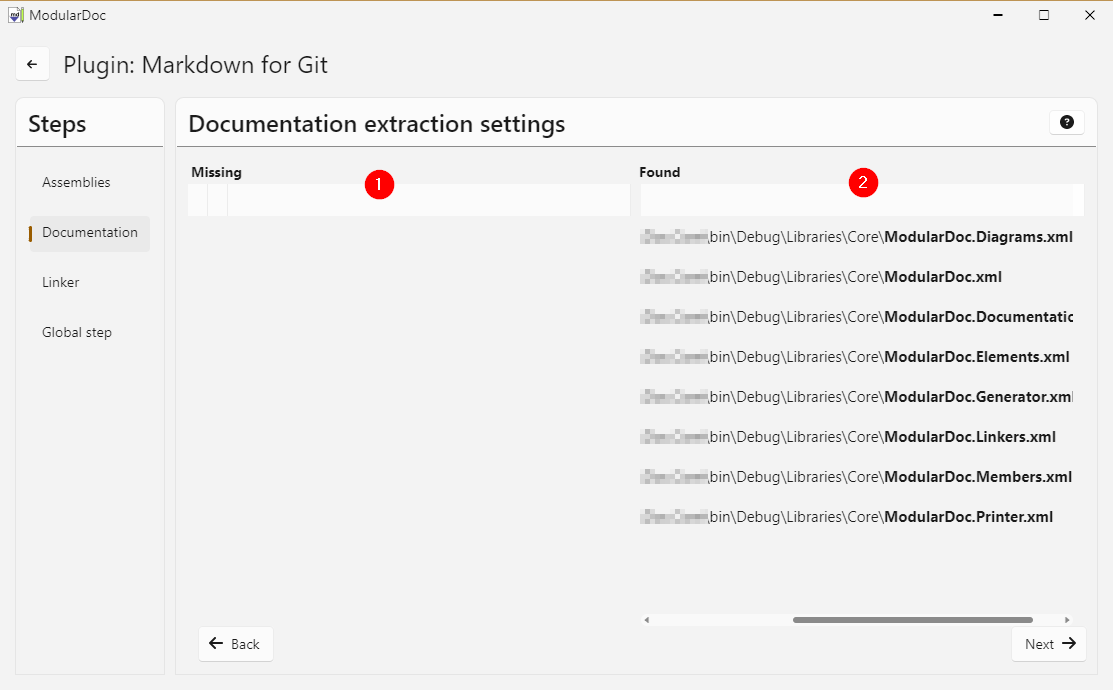
\includegraphics[width=\linewidth]{img/modularDocDocumentation.png}
    \label{fig:modularDocumentation}
    \caption{Plugin documentation configuration step}
\end{figure}

\begin{enumerate}
    \item List of missing documentation files
    \item List of automatically discovered documentation files
\end{enumerate}

\pagebreak
\subsubsection{Linker step}

The linker step is designated for configuring linking settings such that they are valid for the target \ref{gloss:git} hosting platform.

\begin{figure}[H]
    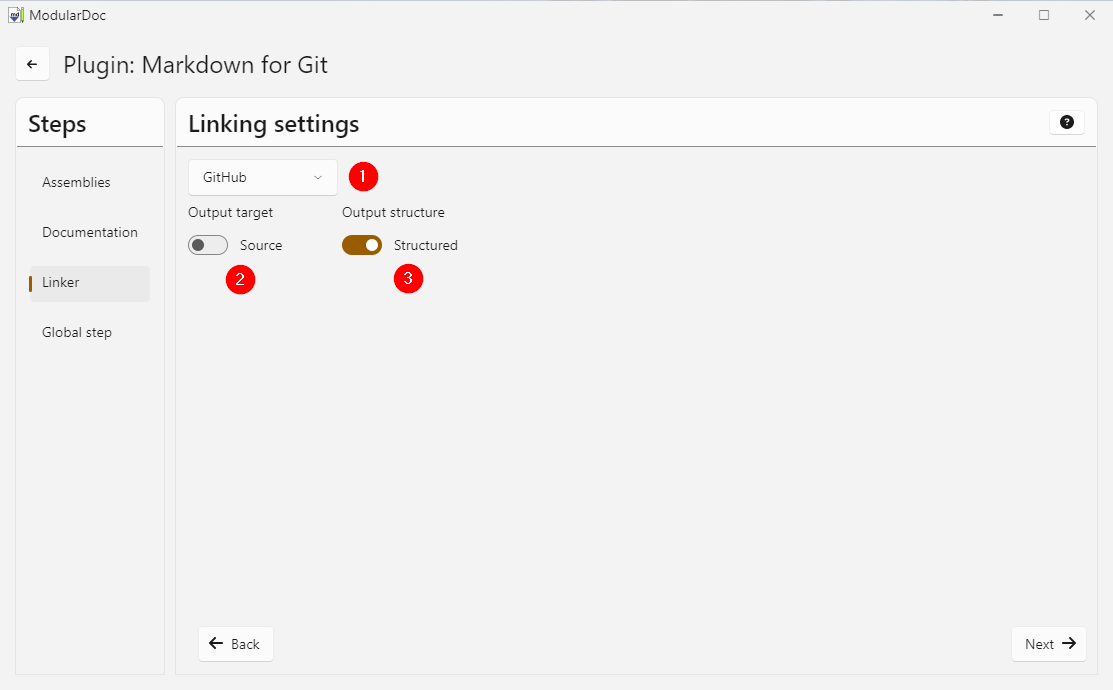
\includegraphics[width=\linewidth]{img/modularDocLinker.png}
    \label{fig:modularLinker}
    \caption{Plugin linker configuration step}
\end{figure}

\begin{enumerate}
    \item Selection of the target platform - GitHub or GitLab
    \item Toggle for the output target - source or wiki
    \item Toggle for the output structure - flat or structured
\end{enumerate}

\pagebreak
\subsubsection{Global step}

The global step is designated for configuring both the generated documentation target output paths, and ignored namespaces and types.

\begin{figure}[H]
    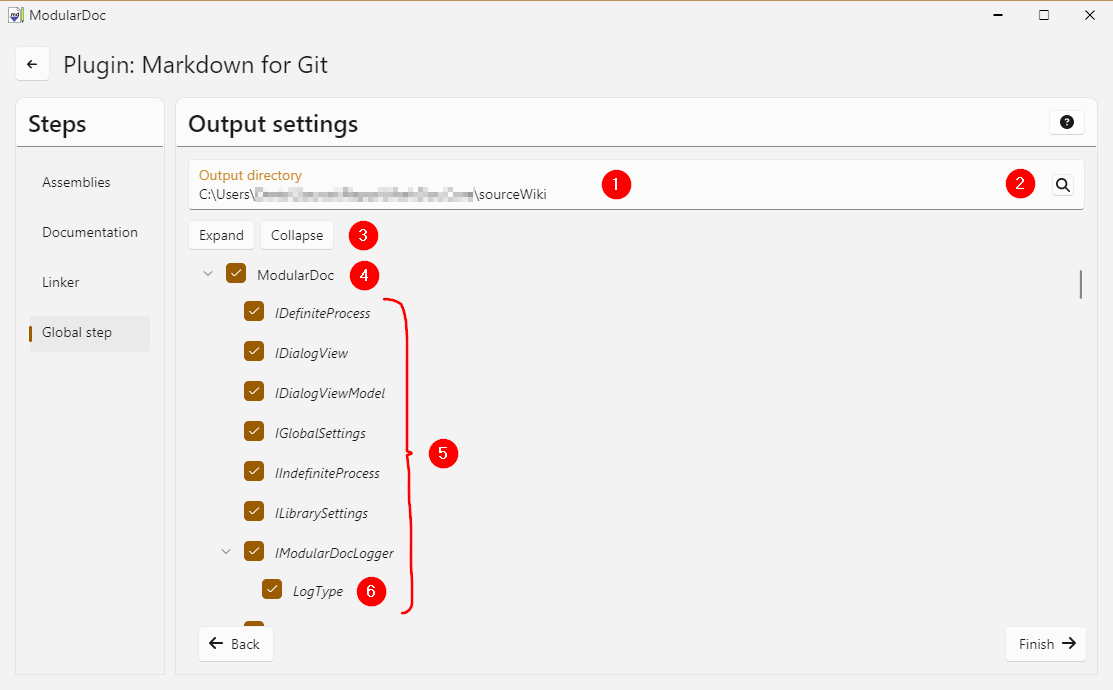
\includegraphics[width=\linewidth]{img/modularDocGlobalSettings.png}
    \label{fig:modularGlobal}
    \caption{Plugin global configuration step}
\end{figure}

\begin{enumerate}
    \item Input field for supplying the generated documentation target output path
    \item Button for opening the folder browser to selected the generated documentation target output path
    \item Buttons for either expanding or collapsing the ignore list
    \item Namespace entry
    \item Type entries
    \item Nested type entry
\end{enumerate}

\subsection{Plugin installation and management}

Plugins are installed by placing them in the \textit{Plugins} folder (see figure \ref{fig:applicationFileStructure}). ModularDoc will automatically load plugins upon startup and display them on the home page. ModularDoc can operate without plugins; however, it loses its purpose.

\section{Developer guide}

\subsection{Prerequisites}

\begin{itemize}
    \item Visual Studio 2019+, JetBrains Rider 2021.3+, or a text editor such as Visual Studio Code is installed
    \item \ref{gloss:dotnetlabel} SDK 6.0.403+ is installed
\end{itemize}

\subsection{Accessing the source code}

This thesis is provided with source for for ModularDoc.
To access the latest source code, clone it from the projects repository on GitHub:

\begin{lstlisting}[caption=Script for cloning the ModularDoc project GitHub repository]
    git clone https://github.com/hailstorm75/ModularDoc.git
\end{lstlisting}

\begin{figure}[H]
    \dirtree{%
    .1 ~ModularDocRepositoryRoot/.
    .2 sourceWiki/.
    .2 src/.
    .3 Components/.
    .4 Diagrams/.
    .4 Documentation/.
    .4 Elements/.
    .4 ....
    .3 Libraries/.
    .4 Core/.
    .4 Helpers/.
    .4 ViewModels/.
    .4 Views/.
    .3 Plugins/.
    .3 ModularDoc.App/.
    .3 ModularDoc.sln.
    .3 ....
    .2 tests/.
    .2 README.md.
    .2 ....
    }
    \caption{ModularDoc simplified source code structure}
    \label{fig:sourceCodeFileStructure}
\end{figure}

Open the \textit{ModularDoc.sln} assembly to start development on the project.
Compiling the solution will generated the \textit{bin/} folder in the root folder.

\subsection{Developing a new component}

Follow these steps to develop a new component:
\begin{enumerate}
    \item Decide which for which key area to develop a new component, e.g. element provider
    \item Create a new project in the respective folder (in this case, \textit{Components/Elements})\linebreak with the following naming scheme - \textbf{ModularDoc.Elements.MY\_COMPONENT}
    \item Configure the project in the same way as one of the other existing provider components
    \item Inherit the respective interface from \textit{Libraries/Core} in the new component (in this case,\linebreak \textit{ModularDoc.Elements})
    \item Based on the interface definitions, implement the new component
\end{enumerate}

\subsection{Developing a new plugin}

Follow these steps to develop a new plugin:
\begin{enumerate}
    \item Create a new project in \textit{Plugins} folder with the following naming scheme - \textbf{ModularDoc.Plugins.MY\_PLUGIN}
    \item Configure the new project in the same way as one of the other existing plugins
    \item Reference the 
    \item Create a type representing the plugin instance and implement the plugin interface from the referenced core library
    \item Create a new project in the \textit{Libraries/ViewModels} folder with the following naming scheme - \textbf{ModularDoc.ViewModels.MY\_PLUGIN}
    \item Configure the new project in the same way as one of the other existing view model projects
    \item Create a new project in the \textit{Libraries/Views} folder with the following naming scheme - \textbf{ModularDoc.Views.MY\_PLUGIN}
    \item Configure the new project in the same way as one of the other existing view projects

\end{enumerate}